%%%%%%%%%%%%%%%%%%%%%%%%%%%%%%%%%%%%%%%%%%%%%%%%%%%%%%%%%%%%%%%%%%%%%%
% Overleaf (WriteLaTeX) Example: Molecular Chemistry Presentation
%
% Source: http://www.overleaf.com
%
% In these slides we show how Overleaf can be used with standard 
% chemistry packages to easily create professional presentations.
% 
% Feel free to distribute this example, but please keep the referral
% to overleaf.com
% 
%%%%%%%%%%%%%%%%%%%%%%%%%%%%%%%%%%%%%%%%%%%%%%%%%%%%%%%%%%%%%%%%%%%%%%
% How to use Overleaf: 
%
% You edit the source code here on the left, and the preview on the
% right shows you the result within a few seconds.
%
% Bookmark this page and share the URL with your co-authors. They can
% edit at the same time!
%
% You can upload figures, bibliographies, custom classes and
% styles using the files menu.
%
% If you're new to LaTeX, the wikibook is a great place to start:
% http://en.wikibooks.org/wiki/LaTeX
%
%%%%%%%%%%%%%%%%%%%%%%%%%%%%%%%%%%%%%%%%%%%%%%%%%%%%%%%%%%%%%%%%%%%%%%

%\documentclass[9pt]{beamer}
\documentclass[9pt, xcolor=dvipsnames]{beamer}

% For more themes, color themes and font themes, see:
% http://deic.uab.es/~iblanes/beamer_gallery/index_by_theme.html
%
\mode<presentation>
{
  \usetheme{Madrid}       % or try default, Darmstadt, Warsaw, ...
  \usecolortheme{seahorse} % or try albatross, beaver, crane, ...
  \usefonttheme{serif}    % or try default, structurebold, ...
  \setbeamertemplate{navigation symbols}{}
  \setbeamertemplate{caption}[numbered]
}


%%\usepackage{natbib}
%\bibliographystyle{plain}
%% make bibliography entries smaller
%%\renewcommand\bibfont{\scriptsize}
%% If you have more than one page of references, you want to tell beamer
%% to put the continuation section label from the second slide onwards
%\setbeamertemplate{frametitle continuation}[from second]
%% Now get rid of all the colours
%%\setbeamercolor*{bibliography entry title}{fg=black}
%%\setbeamercolor*{bibliography entry author}{fg=black}
%%\setbeamercolor*{bibliography entry location}{fg=black}
%%\setbeamercolor*{bibliography entry note}{fg=black}
%% and kill the abominable icon
%\setbeamertemplate{bibliography item}{\bibitem{E}}

% Uncomment to put article, title etc on the same line
%\setbeamertemplate{bibliography entry article}{}
%\setbeamertemplate{bibliography entry title}{}
%\setbeamertemplate{bibliography entry location}{}
%\setbeamertemplate{bibliography entry note}{}

% Replace the abominable icon by [x]
\setbeamertemplate{bibliography item}{\insertbiblabel}

% set biblio entries color
\setbeamercolor*{bibliography entry title}{fg=black}
\setbeamercolor*{bibliography entry author}{fg=black}
\setbeamercolor*{bibliography entry location}{fg=black}
\setbeamercolor*{bibliography entry note}{fg=black}

\usepackage[english]{babel}
\usepackage[utf8]{inputenc}
\usepackage{ragged2e}
%\usepackage[margin=0pt,size=smaller,labelformat=parens,labelsep=space,skip=0pt,indention=0pt,list=false,hypcap=false]{subcaption}
%\usepackage{subfigure}

\usepackage{verbatim}
%\usepackage{tcolorbox}
\usepackage{appendixnumberbeamer}
\usepackage{bm}
\usepackage{caption}
%\usepackage[dvipsnames]{xcolor}
\usepackage{dirtytalk}
\usepackage{multirow}

% On Overleaf, these lines give you sharper preview images.
% You might want to `comment them out before you export, though.
%\usepackage{pgfpages}
%\pgfpagesuselayout{resize to}[%
%  physical paper width=8in, physical paper height=6in]


\graphicspath{{figures/}} % Path to image directory

%\newcommand{\fts}{9pt}  % fontsize
%\newcommand{\bls}{10.7}  % baselineskip

\newcommand{\hreff}[3][blue]{\href{#2}{\color{#1}{#3}}}%

\AtBeginSection{%
	\begin{frame}
		\fontsize{9pts}{12}\selectfont
		\tableofcontents[ 
		currentsubsection,
		sectionstyle=show/shaded, 
		subsectionstyle=show/show/shaded
		]
	\end{frame}
}


% Here's where the presentation starts, with the info for the title slide
\title[DIY Spectrometer]{DIY Spectrometer}
\author[]{Massimiliano Galli (based on Federica Riti's work)}
%   {
%	Florian Eble \\
%	Under the supervision of Jan Stark
%	}
\institute[]{\normalsize{ETH Z\"urich}}
%\date{\today}

\begin{document}

\begin{frame}
  \vspace{0.5cm}
  %\fontsize{10pts}{12}\selectfont
  \titlepage
\end{frame}

% -------------------------------------------------

% These three lines create an automatically generated table of contents.
\begin{frame}{Outline}
  \fontsize{9pts}{12}\selectfont
  \tableofcontents
\end{frame}


% -------------------------------------------------

%\section{Introduction}
%\begin{frame}{Introduction}
%\begin{columns}
%\column{0.6\textwidth}
%(from manual 15)
%A diffraction grating is an optical element which can separate different wavelengths of light. This is rea- lized by employing a material or surface with spa- tially periodic optical constants (refractive index n or absorption coefficient $\mu$).
%When light falls on a diffraction grating, it is bent.
%To find the light intensity behind the grating we use Huygens princi- ple to sum the contributions of the spherical waves- fronts emanating from each grooves to the observa- tion point. 
%The diffraction phenomenon is derived in the far field at an angle $\phi$ from the direction of the incident light. In this direction a maximum of the light intensity is observed when the phase difference $\Delta$ between two neighboring waves is an integer multiple of the wavelength $\lambda$. If g is the groove spacing, i.e. the so-called grid constant, then the phase difference
%\begin{equation}
%	\Delta = g sin \phi
%\end{equation}
%So the condition for a brightness maximum for
%the wavelength $\lambda$ is:
%\begin{equation}
%	p \lambda  = g sin \phi
%\end{equation}
%where p is an integer and is called the order num- ber of the diffraction maximum. If light composed of different wavelengths $\lambda$ falls on the grating, Then a diffraction maximum is created in different direc- tions for each wavelength. This set of maxima, be- longing to different wavelengths, i.e. colors, is called the spectrum.
%The extraordinary importance of diffraction gratings lies in the fact that by measuring the grating con- stant g and the diffraction angle $\phi$, i.e., in principle by simple length measurements, very precise wave- length determinations are possible.
%\column{0.4\textwidth}
%		\begin{figure}
%		\begin{centering}
%			\centering
%			\captionsetup{justification=RaggedRight,margin={0cm,0cm}}
%			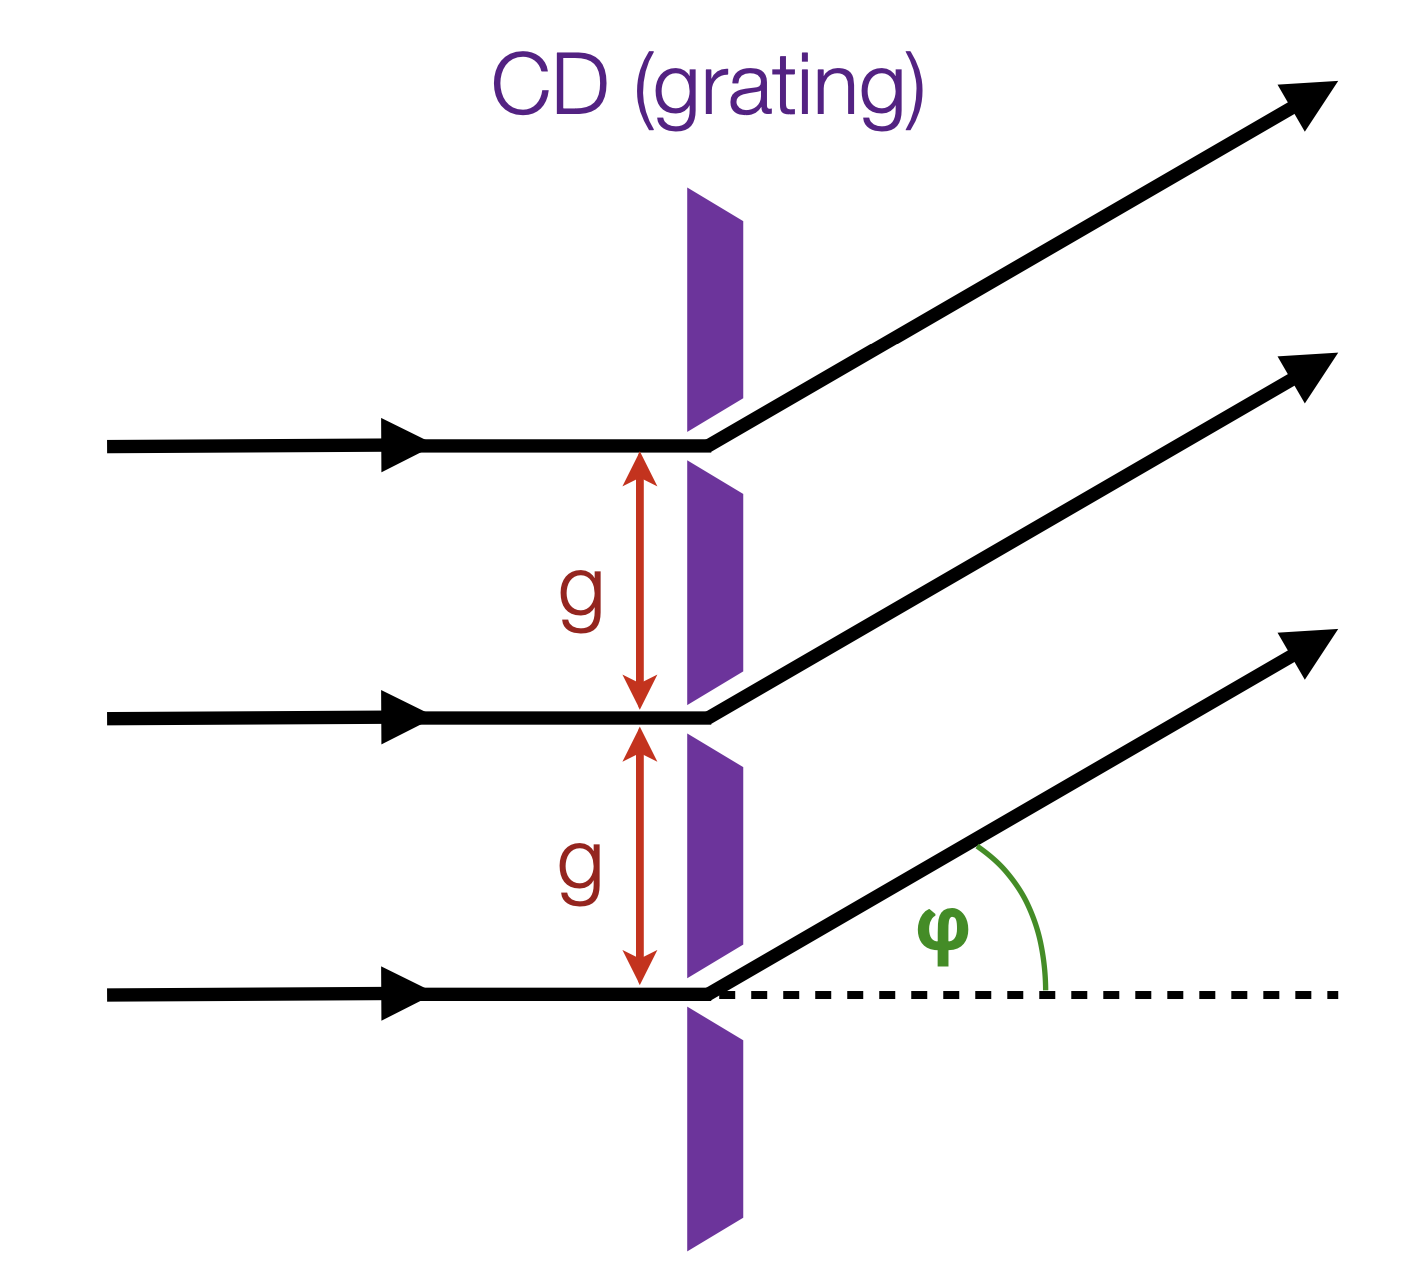
\includegraphics[width=1 \textwidth]{Figures/grid.png}
%		\end{centering}
%		\end{figure}
%	\end{columns}
%\end{frame}

% -------------------------------------------------
\section{Preparation for the lab}


\subsection{Guidelines for the summary }
\begin{frame}{Guidelines for the summary}


\begin{itemize}
	\item Each person should write a summary of the experiment (2 summaries per group);
	\item It should contain a description of the experiment:  the goal etc...
	\item Write it in English;
	\item 1 page maximum;
	\item Save it in PDF format;
	\item Don't copy, write it in your own words;
	\item It must be sent to me by email before the beginning of the lab at this email \hreff{mailto:masgalli@phys.ethz.ch}{masgalli@phys.ethz.ch}.
\end{itemize}


\end{frame}


\subsection{Manual }
\begin{frame}{Manual and other links}

\textbf{Before the lab you need to read the manual carefully}.

~\\

\begin{itemize}
	\item This is the link to the  \textcolor{blue}{\href{https://ap.phys.ethz.ch/}{Praktikum webpage}}, where you can find all the info about the course;
	\item \textcolor{blue}{\href{https://ap.phys.ethz.ch/83.html}{Manual} } for the DIY Spectrometer.
\end{itemize}

~\\


Other useful links that you can also find on the manual:
\begin{itemize}
	\item \textcolor{blue}{\href{https://www.youtube.com/watch?v=fl42pnUbCCA}{Youtube video}} that you can watch to have an idea on how to build the spectrometer;
	\item \textcolor{blue}{\href{https://ieeexplore.ieee.org/stamp/stamp.jsp?tp=\&arnumber=5547333\&tag=1}{Paper }}to (maybe) take grating constant values.\\
	~\\
	\textit{Problems in opening the paper?} 
	\begin{itemize}
		\item You need to be connected with ETH network (either in person or use a VPN)
		\item If you are redirected to another page, the problem is usually due to cookies that are not enabled in the browser: follow the instructions on the website.
	\end{itemize}
\end{itemize}

\end{frame}

\subsection{Material to prepare}
\begin{frame}{Material to prepare}

\textbf{The Material you need to prepare before the lab}.

~\\

\begin{itemize}
\item Cardboard;
\item CD-R that you don’t need (NOT a DVD);
\item scissors or cutter;
\item ruler;
\item razor blades;
\item tape (preferably dark);
\item a smartphone or camera;
\item optional: laser pointer (useful for task 1).

\end{itemize}

~\\
\textit{Suggestion: As you can see from the manual or from the youtube video, you'll need to remove the reflective foil from the CD. I suggest you try to remove it before the lab session, because it may be difficult depending on the CD, and you may need to change it.}



\end{frame}
% -------------------------------------------------

\section{During the lab}

\subsection{Plan for lab session}
\begin{frame}{Plan for lab session}

\textbf{1. Introduction}
\begin{itemize}
	\item Follow this short presentation;
\end{itemize}


\textbf{2. Summaries}

\begin{itemize}
	\item Send the summary to \hreff{mailto:masgalli@phys.ethz.ch}{masgalli@phys.ethz.ch};
\end{itemize}
\textbf{3. Build the Spectrometer}
\begin{itemize}
	\item 1 breakout room for each group;
	\item If member of the same group are not physically in the same room, you must build one spectrometer per person;
	\item If in the same room you can build only one spectrometer per group.
	\item Build the DIY spectrometer:
	\begin{itemize}
	    \item Use Manual directions;
	    \item Take pictures;
	    \item Write down the procedure you follow!
	\end{itemize}
		\end{itemize}

\textbf{4. Do the tasks}

	\begin{itemize}
		\item There are 3 mandatory tasks + an optional one;
		\item Write down measurements you get.
    \end{itemize}


\end{frame}


% -------------------------------------------------
\subsection{Zoom organisation}

\begin{frame}{Zoom organisation}

\textbf{Zoom rooms}
\begin{itemize}
	\item Main zoom room for general announcements;
	\item  I will assign group members to the same breakout room so that you can work together;
	\item If you get kicked out due to the change of room, please reconnect.
\end{itemize}

~\\
\textbf{Communication}
\begin{itemize}

	\item I will come to your room regularly to check how it goes and whether you have questions;
	\item You can always ask for help (there is a button on Zoom called "Ask for Help") at any time if you have a question or need help.
\end{itemize}

\end{frame}

% -------------------------------------------------

\subsection{Build the Spectrometer}
\begin{frame}{Build the Spectrometer}
	\textbf{Box}
	\begin{itemize}
		\item Inside of the box should be non reflective and dark (plain cardboard is fine);
		\item Make sure that no light enter the box apart from the slit.
	\end{itemize}
	\textbf{Slit}
	\begin{itemize}
		\item The slit is made with the two razor blades, and attached to the tube with tape;
		\item The razor blades have to be parallel;
		\item The width of the slit should be of the order of 0.1 mm;
		\item \textit{Suggestion: Build the slit using a piece of paper to separate the razor blades; in this way you can be sure that they are parallel and that the distance is small enough}.
	\end{itemize}
		\textbf{Grating}
	\begin{itemize}
		\item The CD without the foil acts as the grating;
		\item Make sure it's clean enough (you will see also from the quality of the pictures);
		\item Grooves in the CD should be parallel to the slit. \textit{Hint:} the grooves in the CD are concentric.
	\end{itemize}
~\\

\textit{You can start taking the first pictures!}
\end{frame}
% -------------------------------------------------
\subsection{ Tasks - an Overview}
\begin{frame}{Tasks - an Overview}

The experiment is composed of 3 mandatory tasks and an optional one. 
\begin{itemize}
	\item \textbf{Task 1} - Measure the grating constant of the CD;
	\item \textbf{Task 2} - Calibration (measure d);
	\item \textbf{Task 3} - Measure the wavelenght from some other source of light;
	\item \textbf{Task 4} (\textit{Optional}) - Fraunhofer lines.
	\end{itemize}
	
	~\\
	The first two tasks allow you to measure the features of your spectrometer; once that is done, you can point your spectrometer to every light source and measure the wavelengths of the components (Task 3).

\end{frame}
% -------------------------------------------------

\subsection{ Task 1 - Measure the grating constant of the CD}
\begin{frame}{Task 1 - Measure the grating constant of the CD}
\begin{columns}
	\column{0.6\textwidth}
	\begin{itemize}
		\item The goal is to measure the grating constant of the CD;
		\item The formula useful to know for this task is:
	\end{itemize}
	~\\
	\begin{equation}
		p \lambda = g sin \phi
	\end{equation}
	where p=1 is the order number, $\lambda$ is the wavelenght, g is the grating constant and $\phi $ is the diffraction angle.
	
	\column{0.4\textwidth}
		\begin{figure}
		\begin{centering}
			\centering
			\captionsetup{justification=RaggedRight,margin={0cm,0cm}}
			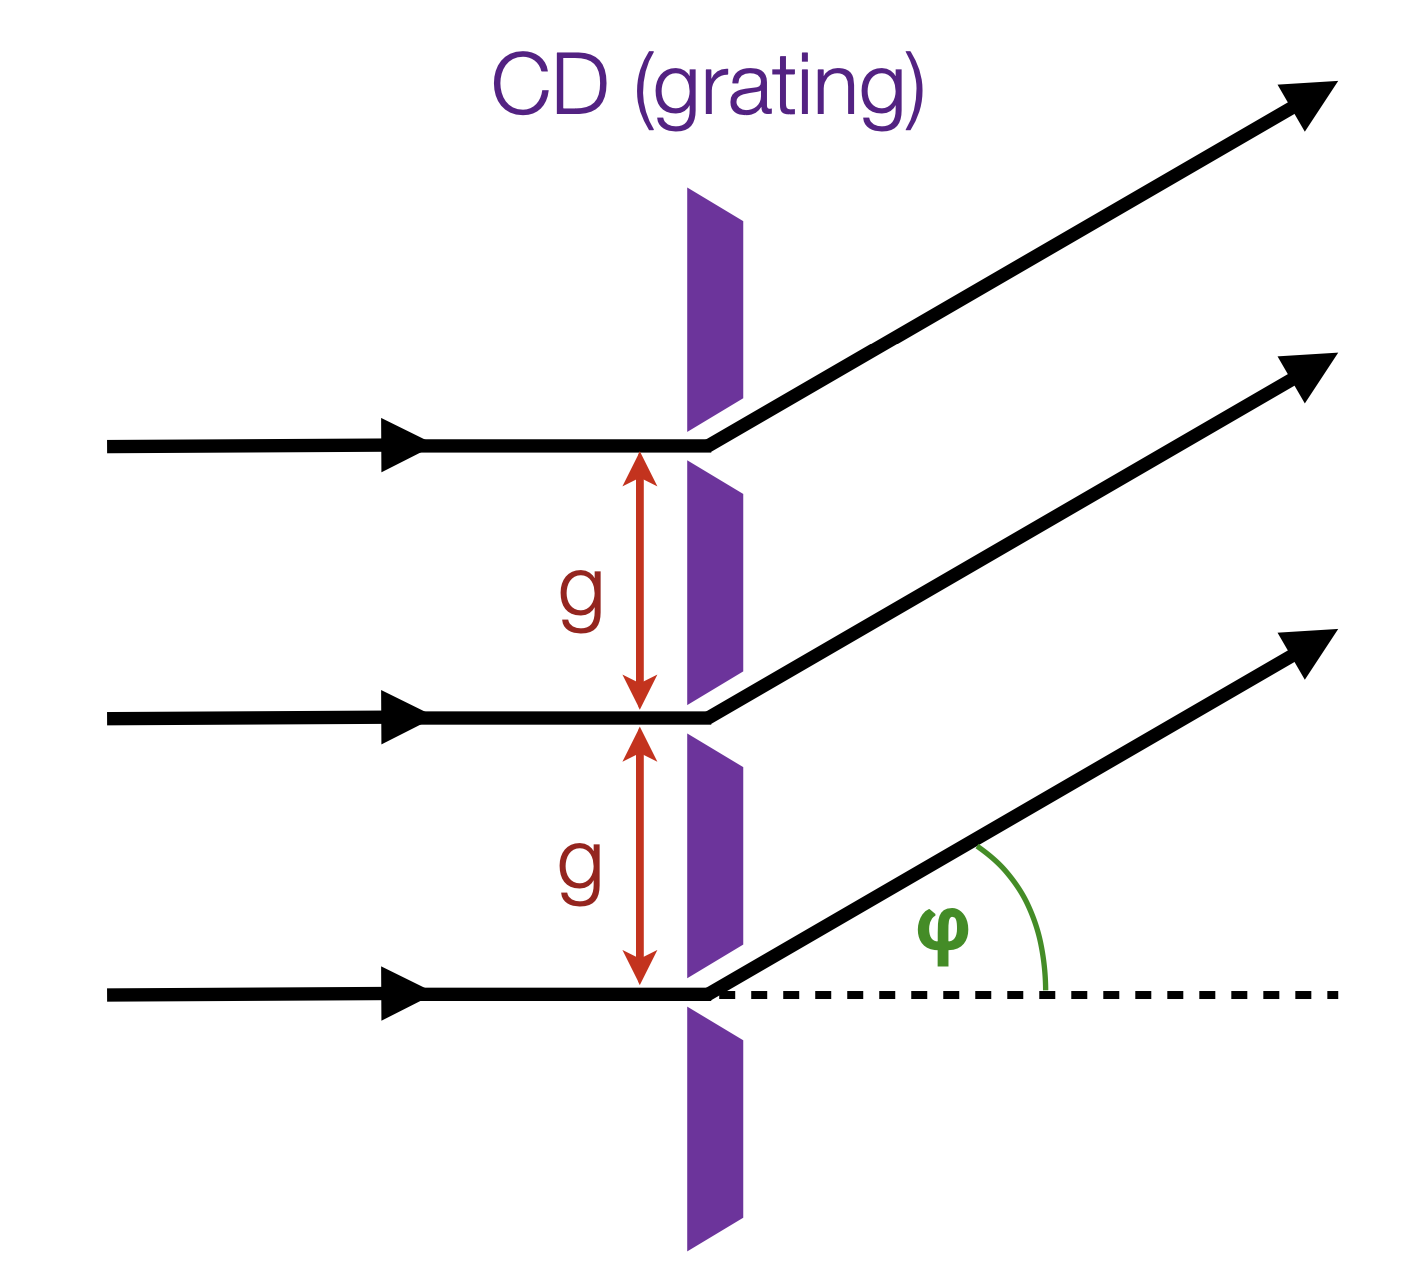
\includegraphics[width=1 \textwidth]{Figures/grid.png}
		\end{centering}
		\end{figure}
	\end{columns}

\end{frame}

\begin{frame}{Task 1 - Measure the grating constant of the CD}	
If we know $\lambda$, we still have two unknown variables in the equation: $g$ and $\phi$.
	
	\begin{equation*}
		 \lambda = g sin \phi
	\end{equation*}
	\begin{columns}
	\column{0.4\textwidth}
	
	How to measure g? There are different ways, here some:
	\begin{itemize}
		\item With a laser pointer: you can measure $\phi$ as in the figure, then you can calculate g.		
		\item If you don't have a laser pointer: depending on the features of your CD, you can find the grating constant from the table in the \textcolor{blue}{\href{https://ieeexplore.ieee.org/stamp/stamp.jsp?tp=\&arnumber=5547333\&tag=1}{paper}}.
	\end{itemize}
	\textit{Suggestion: if you use the laser pointer, you might want to put a piece of paper on the wall in order to write down the position of the light and then measure it with the ruler.}
	\column{0.6\textwidth}
		
		\begin{figure}
		\begin{centering}
			\centering
			\captionsetup{justification=RaggedRight,margin={0cm,0cm}}
			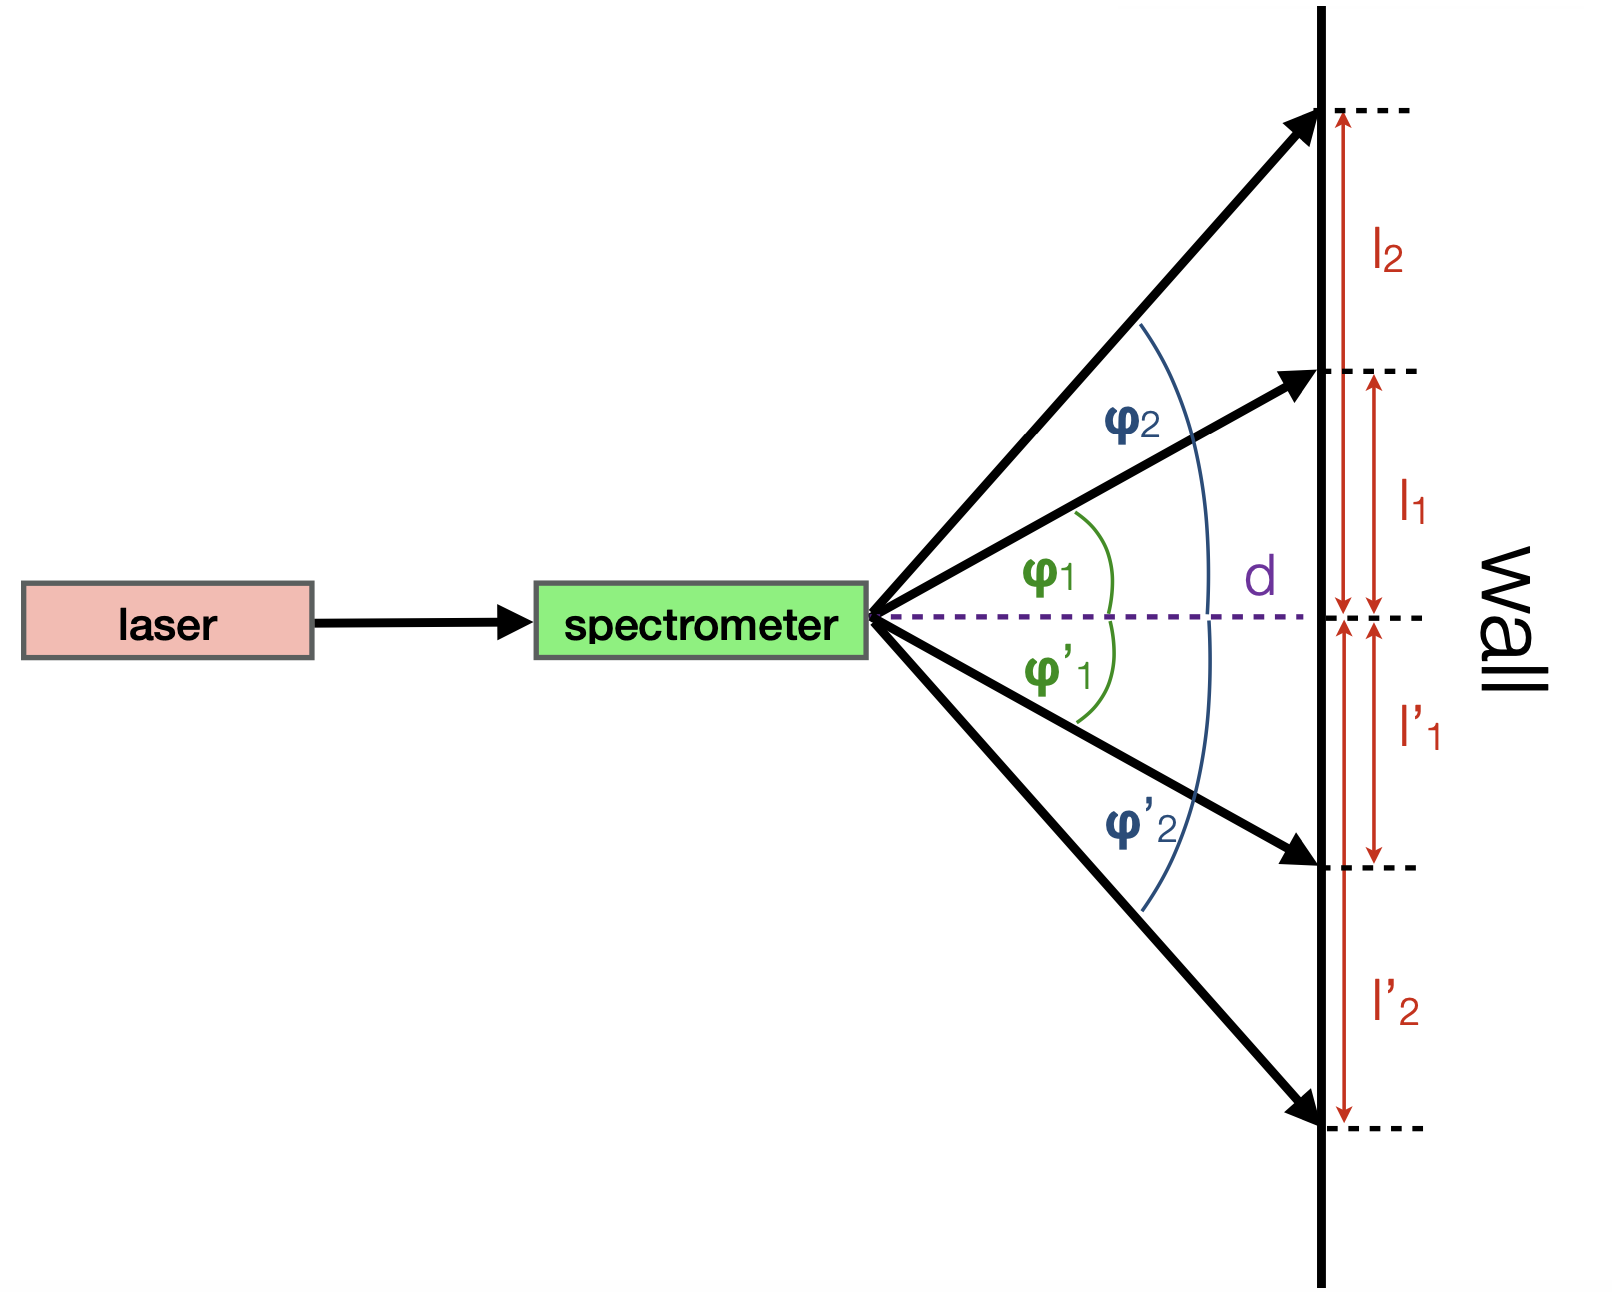
\includegraphics[width=1 \textwidth]{Figures/laser.png}
		\end{centering}
		\end{figure}
\end{columns}
\end{frame}

% -------------------------------------------------
\subsection{ Task 2 - Calibration}

\begin{frame}{Task 2 - Calibration}	
Calibrating the spectrometer means to measure the distance between the grating and the sensor of the camera. It is not a distance you can measure directly, so you need to find a way to calculate it.

~\\
	Knowing $\lambda$ we have two unknown variables in the equation: $g$ and $\phi$. You measured g from Task 1, so you only miss $\phi$.

\begin{equation*}
		 \lambda = g sin \phi
	\end{equation*}
	
	\begin{columns}
	\column{0.6\textwidth}
	How to measure d? 
	\begin{itemize}
		\item You can use again the laser pointer (scheme on the right);
		\item Or you can use the sunlight spectrum (next slide).
	\end{itemize}

	
	\column{0.4\textwidth}
		
		\begin{figure}
		\begin{centering}
			\centering
			\captionsetup{justification=RaggedRight,margin={0cm,0cm}}
			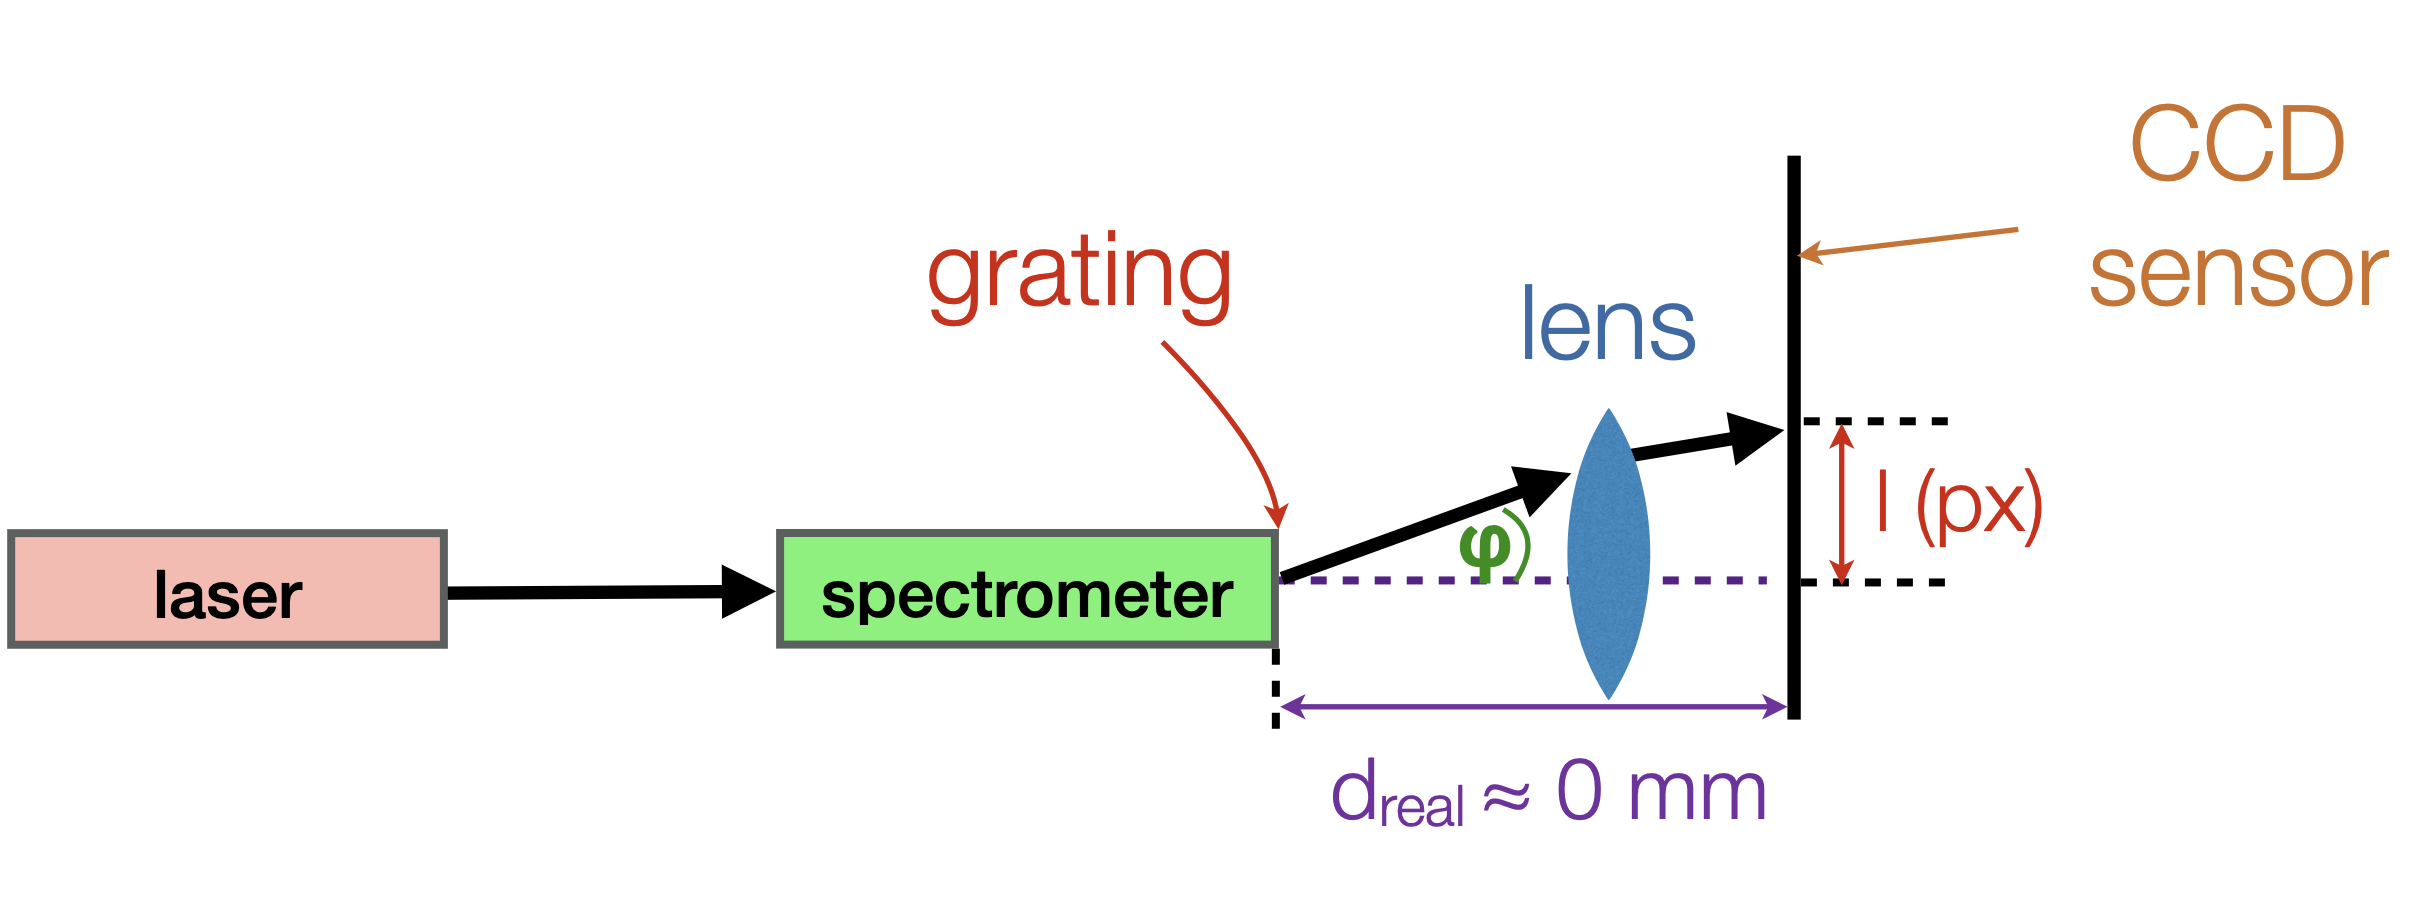
\includegraphics[width=1 \textwidth]{Figures/calibration.png}
		\end{centering}
		\end{figure}
\end{columns}
	
\textit{Note: since only ratios are involved, you don't necessarily need to convert from pixels to mm.}
	
		
\end{frame}

\begin{frame}{Task 2 - Calibration}	
\centering
	\textbf{How do we measure d from the sunlight spectrum?}
	\begin{columns}
	\column{0.6\textwidth}
\begin{equation*}
		 \lambda = g sin \phi
	\end{equation*}
	\begin{itemize}
		\item Take a picture of what you see in the spectrometer if you point it to the sunlight;
		\item Measure the distance $x$ (in pixels) between the slit and the color line you decided to measure (choose a narrow color band, like cyan or orange);
		\item  To measure you need to analyse the picture on your computer (PowerPoint or any image processor);

			\end{itemize}
	\column{0.4\textwidth}
		
		\begin{figure}
		\begin{centering}
			\centering
			\captionsetup{justification=RaggedRight,margin={0cm,0cm}}
			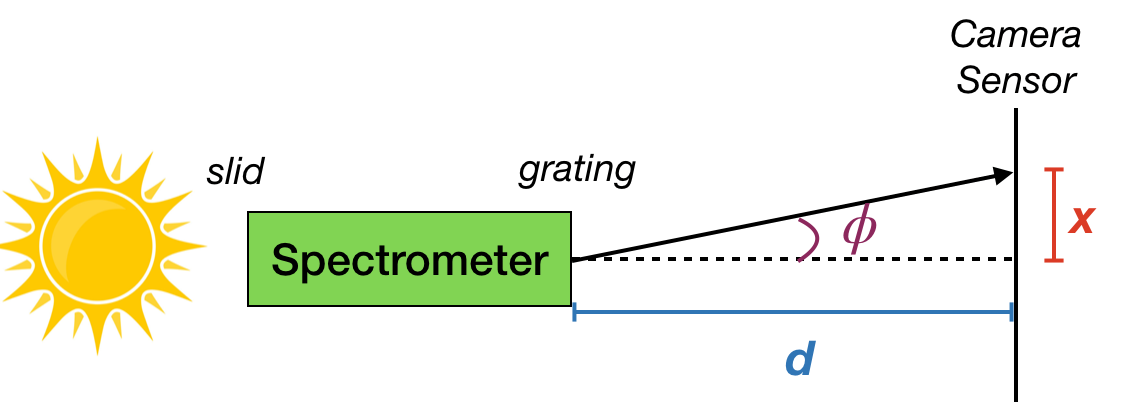
\includegraphics[width=1 \textwidth]{Figures/scheme.png}
			\quad
			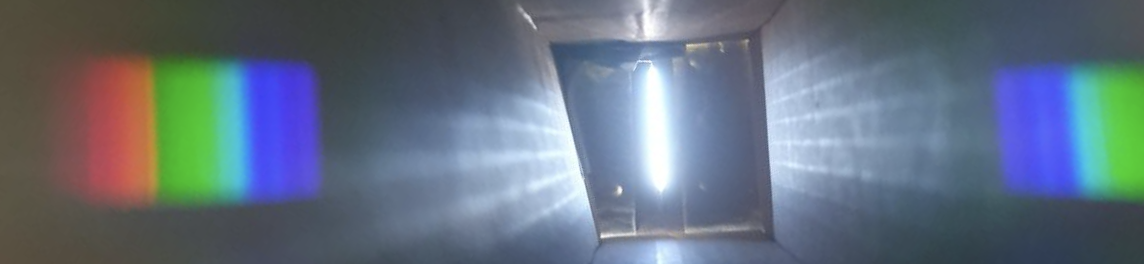
\includegraphics[width=1 \textwidth]{Figures/sunlight.png}
			\quad
			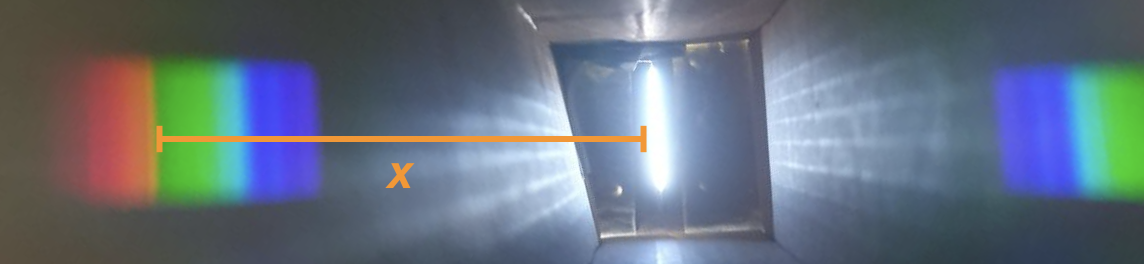
\includegraphics[width=1 \textwidth]{Figures/x.png}
			

		\end{centering}
		\end{figure}
\end{columns}

	

	\begin{itemize}
		\item How to estimate the \textbf{uncertainty} on $x$? Go to Section 3 of these slides;
		\item You can keep all your measurements in pixels, OR you can convert them in mm (but be careful with the uncertainties!);
		\item Now that you measured $x$, you can calculate $d$ as a function of $\lambda, x, g$! Remember to propagate the uncertainties!

	\end{itemize}
	
	
\end{frame}
% -------------------------------------------------
\subsection{ Task 3 - Take Pictures of different light sources}

\begin{frame}{Task 3 -  Take Pictures of different light sources}	
Now your spectrometer is completely calibrated: you know both its grating constant g and the effective distance $d$. \\
It's now time to use it for its purpose: \textbf{measure some wavelenghts}!

~\\

	Take pictures of	 different light sources and see what you find.

~\\
	\begin{columns}
	\column{0.6\textwidth}
	\begin{itemize}
		\item Take pictures of the white light on your laptop, what do you see?

		\item Let's use again the equation $\lambda = g sin \phi$. Measure the $x$ in pixels for blue (or another color) and calculate $\lambda$ (with its uncertainty). Now compare it with the actual wavelenght of $\lambda_{blue}$.
		
		\item Take pictures of other light sources and/or from different colors (see \hreff{https://www.ledr.com/colours/multi.htm}{this} website).
	\end{itemize}
	\column{0.4\textwidth}
	\begin{figure}
		\begin{centering}
			\centering
			\captionsetup{justification=RaggedRight,margin={0cm,0cm}}
			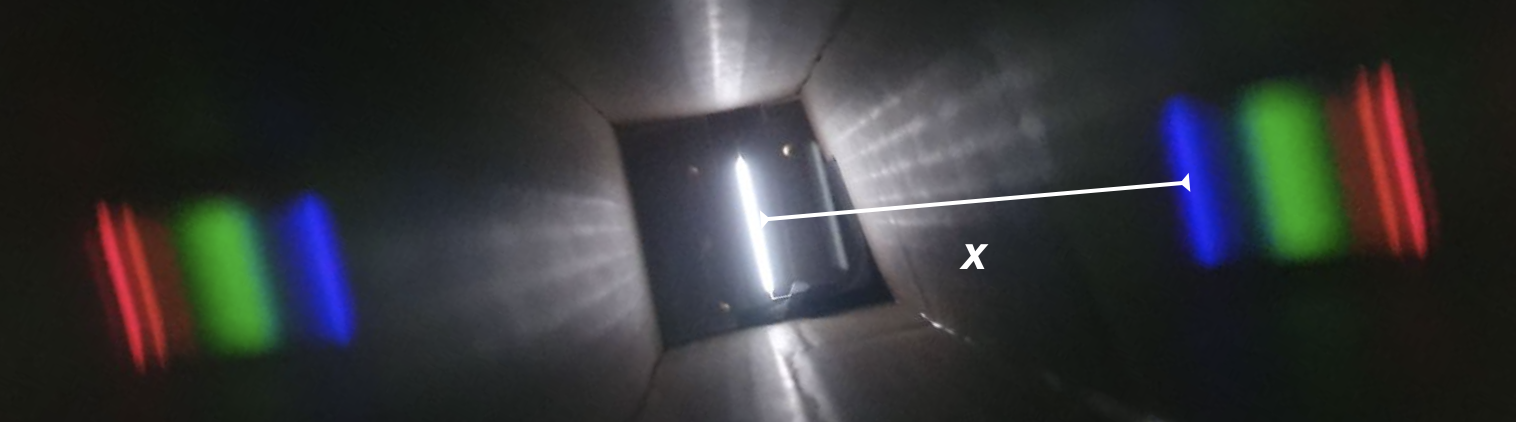
\includegraphics[width=1 \textwidth]{Figures/laptop.png}
		\end{centering}
		\end{figure}
\end{columns}
	\end{frame}

% -------------------------------------------------
\subsection{ Task 4 (Optional) - Fraunhofer Lines}

\begin{frame}{Task 4 - Fraunhofer Lines}	
This is an optional task: not everyone can see the 	Fraunhofer lines, because of the camera or the spectrometer.

~\\

\begin{itemize}
	\item Can you see the Fraunhofer lines?
	\item Can you measure the corresponding wavelenght of some of them?
	
\end{itemize}

~\\
~\\

\centering

Do you have another idea that you want to try? \\
Do it and document it in the report!

\end{frame}

% -------------------------------------------------

\subsection{Report }


\begin{frame}{Report }
You need to write a report of the experiment. \\
Only 1 report per group is required.

~\\

\textbf{General content of the report:}
\begin{itemize}
    \item Descriptions of the experimental setup (two if you are NOT in the same room)
    \item Measurement  (two if you are NOT in the same room)
    \item Analysis of the measurements.
\end{itemize}

~\\
\textbf{Requirements:}
\begin{itemize}
    \item See minimal requirements \hreff{https://p.phys.ethz.ch/WeitereDoks/MinimalRequirementsReport.pdf}{here}\\
    \begin{itemize}
        \item Units
        \item Meaningful number of significant digits
        \item Measurement uncertainties, error propagation
        \item Explain your data analysis and error calculations
    \end{itemize}
    \item The report must written in English
    \item The report must NOT be hand-written. You can use a Word Processor or try Latex! (you can use \hreff{https://www.overleaf.com/}{Overleaf}) Send the report as a PDF.
    \item Send me the report by email at \hreff{mailto:masgalli@phys.ethz.ch}{masgalli@phys.ethz.ch} before next Tuesday noon (12:00 am).
\end{itemize}
\end{frame}

\begin{frame}{Report }
\textbf{Some guidelines:}
~\\
\begin{itemize}
    \item Introduction with a brief theoretical discussion about the experiment (see also \textcolor{blue}{\href{https://ap.phys.ethz.ch/Anleitungen/Bilingual/15_Manual.pdf}{manual}} of experiment 15) ;
    \item Write clearly your measurements and their uncertainties: How did you measure it? How did you find the associated uncertainty? Which numbers have you measured?
    \item When you do calculations, all the formulas you use have to be written in the report, explaining what you are doing. The numbers should be put only at the end!
    \item When you calculate a variabile, you need to propagate the uncertainty. Use the guidelines in Section 3 of these slides. Write the final formula of your propagation on the report!
    \item Always remember to write the units.  
    \item Write the bibliography. Where have you taken the g value? Where do the concepts of the introduction come from? etc...
\end{itemize}


\end{frame}
\subsection{Self - Evaluation }

\begin{frame}{Report - self evaluation}

\begin{figure}
		\begin{centering}
			\centering
			\captionsetup{justification=RaggedRight,margin={0cm,0cm}}
			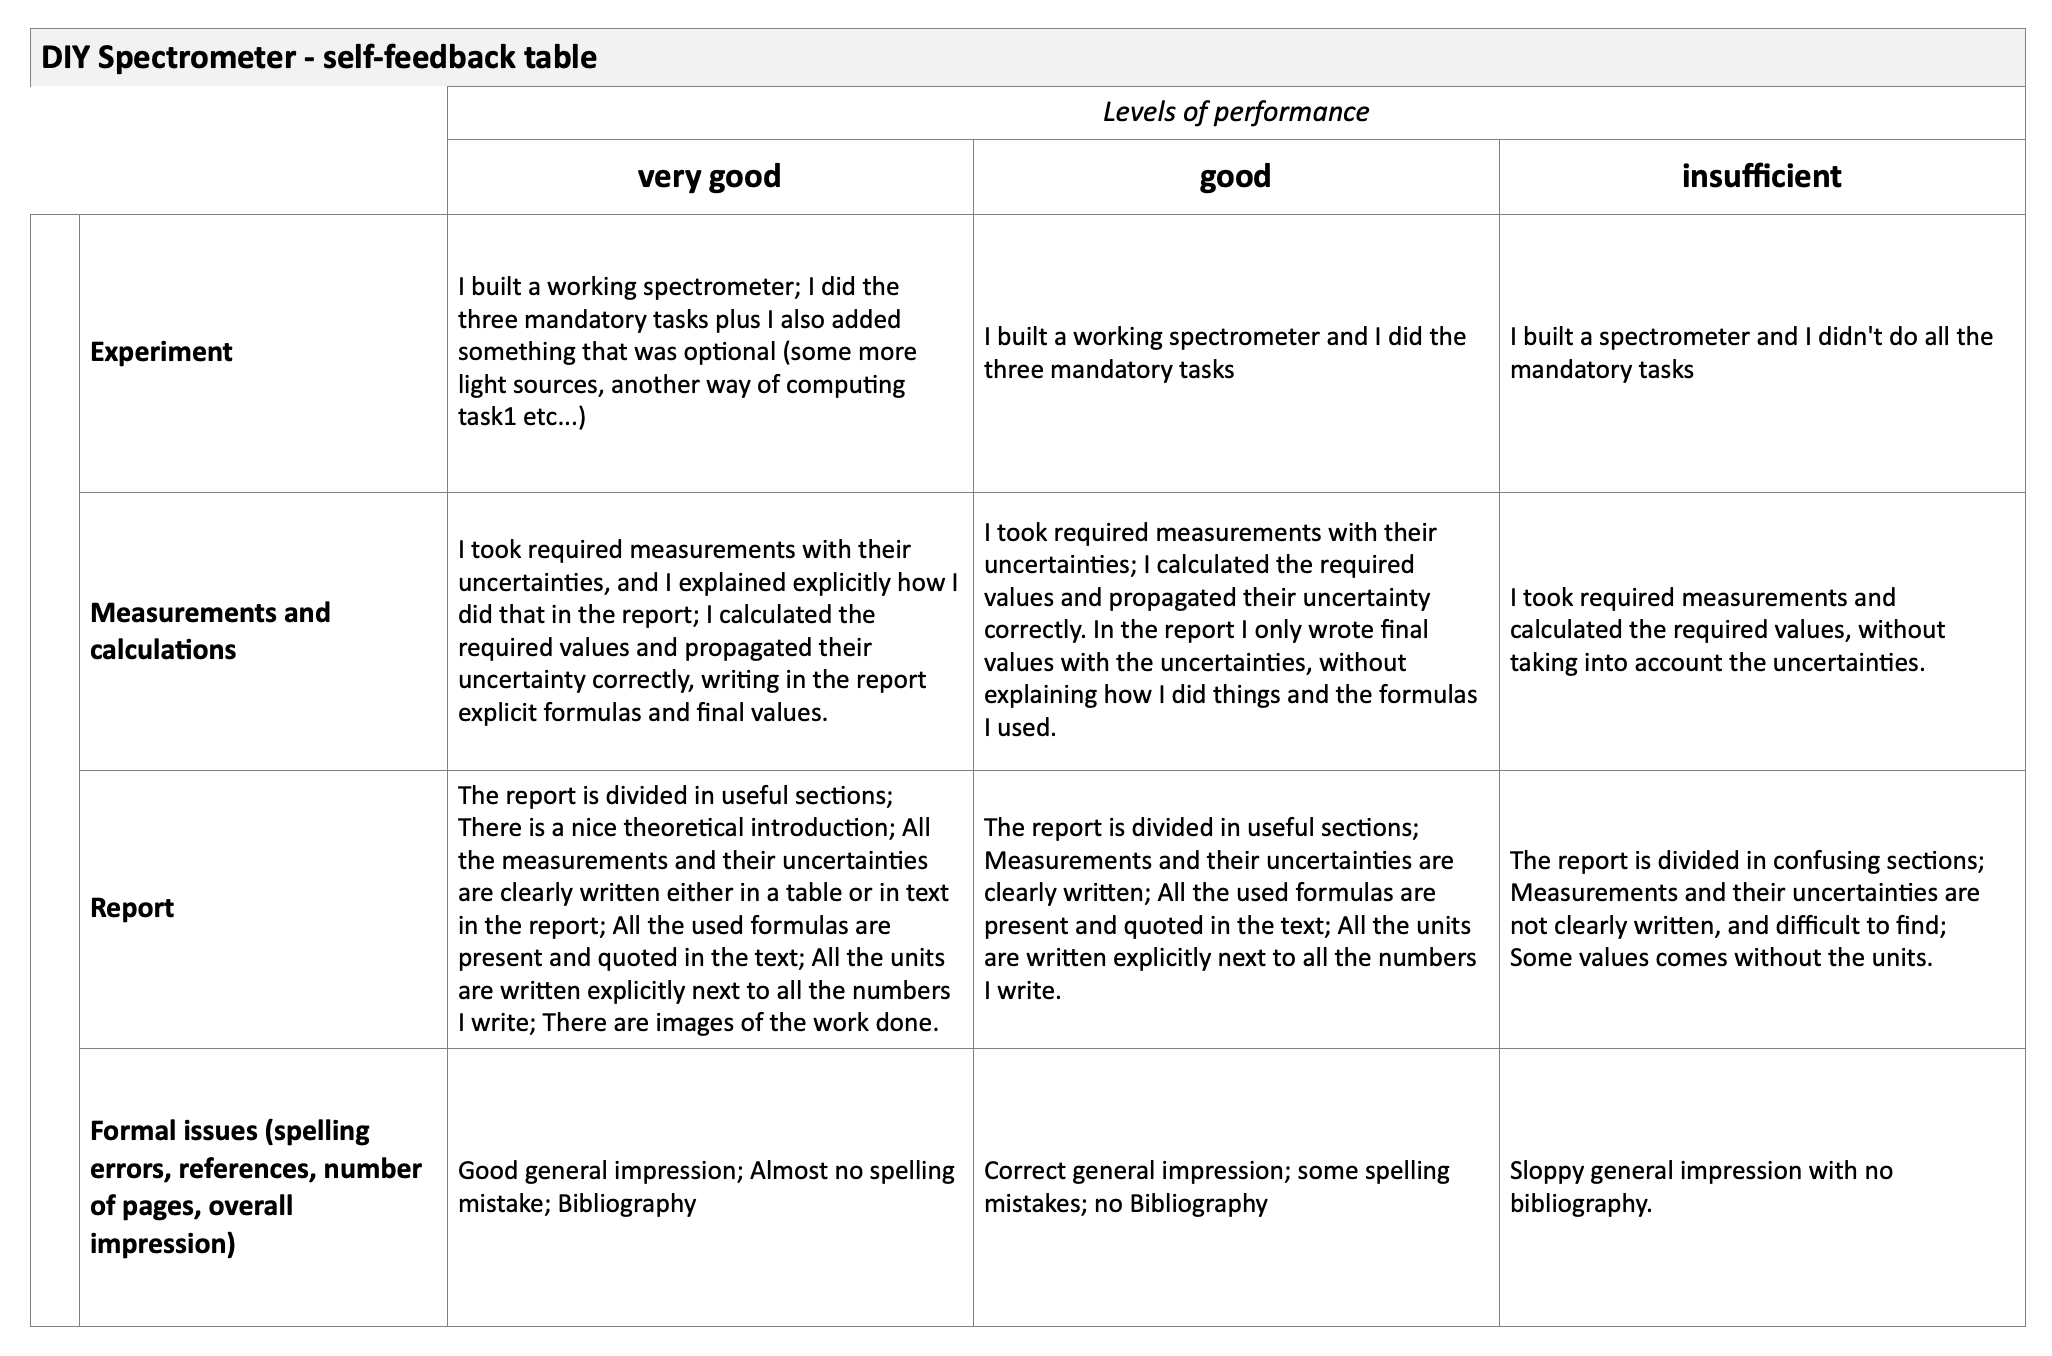
\includegraphics[width=1 \textwidth]{Figures/selffeedbacktable.png}
		\end{centering}
		\end{figure}

\end{frame}

% -------------------------------------------------


\section{Measurement uncertainties}





\subsection{Uncertainty on a single measurement}

\begin{frame}{Uncertainty on a single measurement }
%The uncertainty on a single measure $x$ depends on the instrument you use to measure it. 
%	
%	If you want to measure the width of a box with a ruler, whose smaller unit is the $mm$, you measurement is going to have an uncertainty of $\pm 1mm$, because you can not be more precise than that.
%	
%	~\\
\begin{columns}
	
	\column{0.6\textwidth}

	In our experiment, we measure distances in pixels. For example (in figure) you want to measure the distance between the slit and the blue band of the RGB spectrum. The blue band is thicker than 1 pixel, than you want to estimate an uncertainty that takes that into account. For example, if the distance $x$  is between 200px and 220px, the result will be $x = 210px \pm 10px$.
	
		
	\column{0.4\textwidth}
	\begin{figure}
		\begin{centering}
			\centering
			\captionsetup{justification=RaggedRight,margin={0cm,0cm}}
			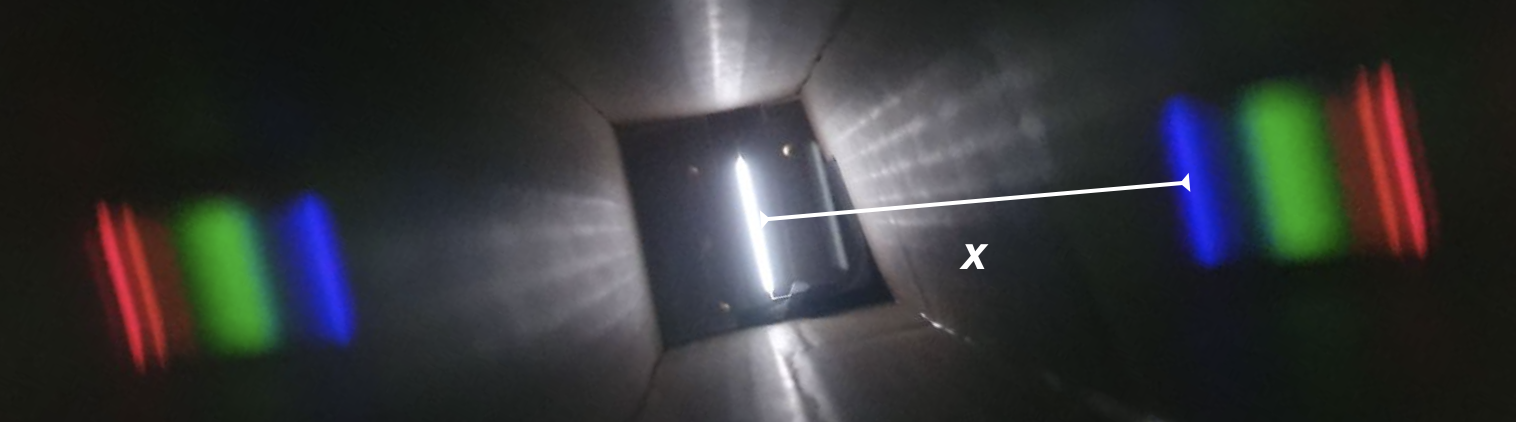
\includegraphics[width=1 \textwidth]{Figures/laptop.png}
		\end{centering}
		\end{figure}
\end{columns}
		
		
\end{frame}

% -------------------------------------------------
\subsection{Linear uncertainty propagation}

\begin{frame}{Linear uncertainty propagation}
	\justify
	In order to estimate the uncertainty on $y = f(x_1, ..., x_n)$, depending on the independent quantities $x_1, ..., x_n$ having uncertainties $\Delta x_1, ..., \Delta x_n$.\\
	The linear uncertainty propagation formula is:
	\begin{equation}
		\Delta y = \sqrt{ \sum_{i=1}^{n} \left(\frac{\partial f}{\partial x_i}\right)^2 \left(\Delta x_i\right)^2 }
		\label{eq:uncertainty_propagation}
	\end{equation}
	
	~\\
	We measure $x = x_0  \pm \Delta x$, and $\Delta x \ll x_0$.
	
	~\\
	\textbf{Question.} What is the uncertainty on $x^2$?
	\begin{itemize}
		\item[] a) $\Delta \left(x^2\right) = \Delta x$
		\item[] b) $\Delta \left(x^2\right) = \left(\Delta x\right)^2$
		\item[] c) $\Delta \left(x^2\right) = 2 x_0 \Delta x$
		\item[] d) I don't know
	\end{itemize}

    ~\\
    ~\\
    ~\\
    \vspace{0.05cm}

\end{frame}


% -------------------------------------------------

\begin{frame}{Linear uncertainty propagation}
	\justify
	In order to estimate the uncertainty on $y = f(x_1, ..., x_n)$, depending on the independent quantities $x_1, ..., x_n$ having uncertainties $\Delta x_1, ..., \Delta x_n$.\\
	The linear uncertainty propagation formula is:
	\begin{equation}
	\Delta y = \sqrt{ \sum_{i=1}^{n} \left(\frac{\partial f}{\partial x_i}\right)^2 \left(\Delta x_i\right)^2 } \tag{\ref{eq:uncertainty_propagation}}
	\end{equation}
	
	~\\
	We measure $x = x_0  \pm \Delta x$, and $\Delta x \ll x_0$.
	
	~\\
	\textbf{Question.} What is the uncertainty on $x^2$?
	\begin{itemize}
		\color{lightgray}
		\item[] a) $\Delta \left(x^2\right) = \Delta x$
		\item[] b) $\Delta \left(x^2\right) = \left(\Delta x\right)^2$
		\color{black}
		\item[] c) $\Delta \left(x^2\right) = 2 x_0 \Delta x$
		\color{lightgray}
		\item[] d) I don't know
	\end{itemize}
	

	
\end{frame}

% -------------------------------------------------
\subsection{Standard Error of the Mean}

\begin{frame}{Standard Error of the Mean }
\textit{You don't need this for the experiment, just for your knowledge...}
	\justify
	We measure $N = 20$ times the same quantity $x$ (e.g. the period of the pendulum) of (unknown!) mean $\mu$ and standard deviation $\sigma$ in the same experimental conditions (e.g. the length of the pendulum does NOT change). We have a series of measurements $x_1, x_2, ..., x_N$ with  empirical mean $\bar{x}$ and standard deviation $s$.
	\newline
	
	\begin{columns}
		\column{0.0\linewidth}
		\column{0.58\linewidth}
		
		Recall that:
		\begin{itemize}
			\item $\bar{x} = \frac{1}{N} \sum_{i=1}^{N} x_i$ \\
			\item $s = \sqrt{ \frac{1}{N-1} \sum_{i=1}^{N} (x_i-\bar{x})^2 }$
		\end{itemize}
		
		~\\
		\textbf{Question 1.} What is the uncertainty on $\bar{x}$?
		\begin{itemize}
			\item[] a) $s$ at 68\% CL (confidence level)
			\item[] b) $2s$ at 95\% CL
			\item[] c) $s/\sqrt{N}$ at 68\% CL
			\item[] d) $2s/\sqrt{N}$ at 95\% CL
			\item[] e) I don't know
		\end{itemize}
		
		\column{0.42\linewidth}
			
		~\\
		~\\
		~\\
		~\\
		~\\
		~\\
		~\\
		~\\
		~\\
		~\\
		~\\
		~\\
		~\\
		~\\
		~\\				
	\end{columns}
	
\end{frame}
%\section{Common Mistakes}
% aggiungi una sezione con i common mistakes, più che altro per me, non da fare vedere a loro
% -------------------------------------------------


% -------------------------------------------------

%\begin{frame}{Bibliography}
%	
%	\textbf{References}
%	
%	\small
%	\bibliographystyle{plain}
%	\bibliography{biblio}	
%	
%\end{frame}


% -------------------------------------------------

%\begin{frame}{}
%	
%
%\end{frame}



\end{document}



%begin{itemize}
%  \item a
%\end{enumerate}
